\subsection{Strategy}
Viene utilizzato quando si ha un gruppo di algoritmi e si vuole poter scegliere l'algoritmo da adottare a runtime.
\begin{figure}[ht]
    \centering
    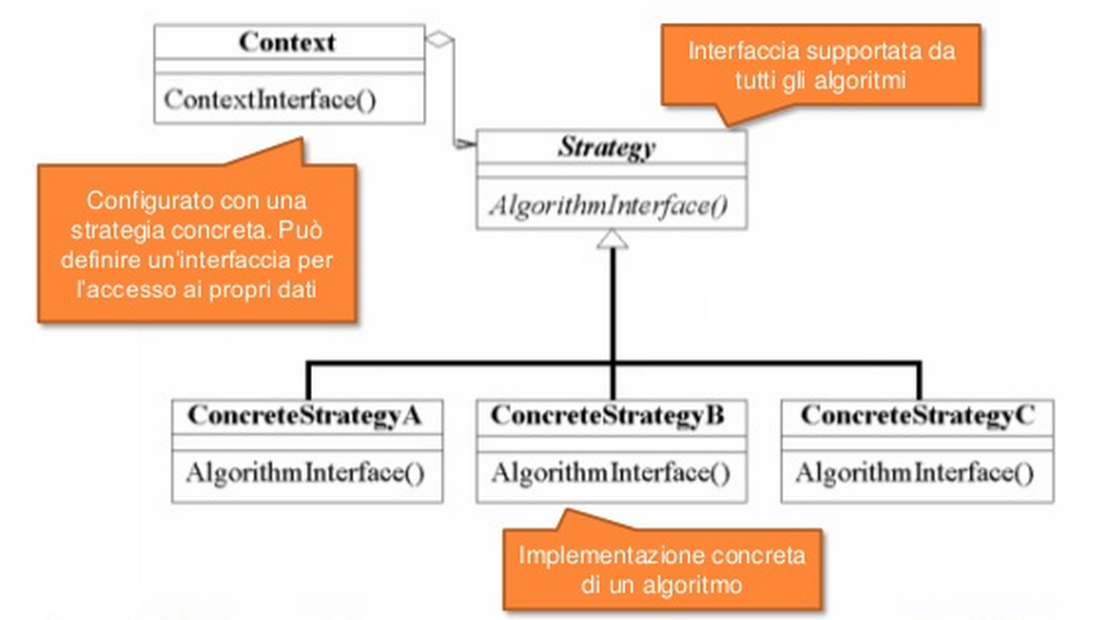
\includegraphics[width=0.8\textwidth]{immagini/strategy.png}
    \caption{Strategy}
\end{figure}
\FloatBarrier
In questo modo è anche più semplice inserire un nuovo algoritmo più efficiente, infatti, basta creare una nuova classe che lo implementa.

\subsubsection{Casi tipici}
\begin{itemize}
\item L'unica differenza tra varie classi correlate è il comportamento;
\item Sono necessarie più versioni di uno stesso algoritmo;
\item Gli algoritmi accedono o utilizzano dei dati che il codice client non deve conoscere;
\item Il comportamento di una classe deve essere definito a runtime.
\item Quando una classe definisce una serie di differenti comportamenti condizionali\footnote{Quando ci sono tanti if per scegliere l'algoritmo effettivo}.
\end{itemize}
